
    The previous chapter introduced a computational idiom --
    Complex Reduction and Histogram Computations (CReHCs) -- and showed how the
    Idiom Description Language (IDL) enables its discovery and automatic
    parallelisation.
    This chapter takes a broader view of automatic idiom detection that also
    includes common sparse and dense linear algebra computations and stencil
    codes.
    Instead of implementing bespoke parallelisation passes, the chapter
    follows the vision laid out in the introduction, using the detection results
    to relevant program parts into stronger models.
    Existing tools are then used to leverage the implied domain knowledge.

    The goal of this chapter is to take abstract algorithmic concepts, which are
    conventionally explored outside the context of compiler analysis --
    computational idioms -- and to formalize them as IDL specifications,
    enabling detection and manipulation in optimising compilers.
    Heterogeneous acceleration will serve as the motivation for this effort.
    As many scientific codes are structured around idiomatic performance
    bottlenecks, efforts that focus on computational idioms can greatly
    improve performance, especially with accelerators that were designed
    with similar computations in mind.
    The focus is therefore on calculations that are well supported by
    accelerators and their software ecosystems: linear algebra,
    stencil codes and CReHCs.

    The IDL specifications are used to build a prototype compiler that
    automatically detects the idioms and uses them to circumvent the code
    generator with libraries and domain specific languages:
    BLAS implementations, cuSPARSE, clSPARSE, Halide and Lift.
    The funcionality is directly accessible in a modified version of the widely
    used Clang C/C++ compilers.
    The evaluation can therefore be performed on the well established benchmark
    suites NAS and Parboil, where 60 idiom instances are detected.
    In those cases where idioms are a significant part of the sequential
    execution time, the generated heterogeneous code achieves 1.26$\times$ to
    over 20$\times$ speedup on integrated and external GPUs.

\section{Introduction}

    Heterogeneous accelerators provide the potential for superior performance.
    However, realising this potential in practice is difficult and requires
    significant programmer effort.
    Programs have to be partially rewritten to target heterogeneous systems,
    using a diverse range of broad and narrow interfaces.
    General-purpose languages such as OpenCL \citep{nvidia11guide} provide
    some portability across heterogeneous devices, but the achieved performance
    often disappoints \citep{lee09openmp}.
    Despite the functional portability, rewrites are required in practice to
    achieve competitive performance.
    Optimised numerical libraries provide more reliable performance, but they
    are more specialised and often provided by hardware vendors without
    portability in mind \citep{clblas,cublas,cusparse,clsparse}.
    More narrow domain-specific languages (DSLs) have been proposed by
    \citet{Ragan-Kelley2013Halide,Franchetti09OL,Rompf:2012:LMS:2184319.2184345}
    among others in attempts to deliver both portability and performance.
    However, this class is quickly evolving, and with most of these DSLs being
    academic projects, the adoption and long term support remain unclear.

    Hardware is becoming increasingly heterogeneous, most recently with the
    development of deep neural network accelerators such as the Google TPU
    \citep{jouppi2017datacenter}.
    This means that library or DSL based programming is likely to become far
    more common.
    The problems with this trend that arise due to the aforementioned tradeoffs
    are evident:
    Firstly, application developers have to learn multiple specialised DSLs and
    vendor-specific libraries if they want good performance.
    Secondly, they will have to rewrite their existing applications to use them.
    Thirdly, this ties code into an ecosystem with unclear future support
    that might soon become obsolete.
    This situation is a severe impediment to the wide-spread efficient
    exploitation of heterogeneous hardware.

    The ideal would be a compiler that automatically maps existing code to
    heterogeneous hardware, with full performance and requiring no directions
    from the application programmer.
    While this is unrealistic in general, the chapter presents a system that
    approximates such a general-purpose system by utilising know-how that is
    already available and encapsulated in the existing backend interfaces.
    Instead of implementing code generation for each heterogeneous
    accelerator, the system maps user code to heterogeneous hardware using the
    existing libraries and domain-specific languages, effectively outsourcing
    the code generation to hardware and domain specialists.

    The approach is based on detecting specific {\em computational idioms} in
    application code that correspond to the functionality of existing interfaces
    -- libraries and DSLs -- for heterogeneous acceleration.
    In addition to the Complex Reduction and Histogram Computations (CReHCs)
    introduced in \Cref{chapter:reductions}, the focus is on
    sparse and dense linear algebra, as well as stencils.
    The covered idioms are a reflection of both the most relevant program
    bottlenecks and the available interfaces.
    Some computational idioms are more widely supported than others, potentially
    pointing to gaps in the accelerator landscape, but some backend was
    available for each of them.
    The Idiom Detection language (IDL) then enabled the automatic detection of
    idioms.

    Once detected, the idioms are mechanically translated into the appropriate
    DSL or replaced with a library call.
    This optimised code, or the pre-built optimised library, is then linked into
    the original program.
    As backends, the libraries cuSparse, clSparse, cuBLAS, clBLAS for
    sparse and dense linear algebra and target the DSL Halide
    \cite{Ragan-Kelley2013Halide} for stencil computations are used in the
    evaluation.
    In addition to this, the Lift language \cite{SteuwerRD17} is used - a data
    parallel language that supports generalized reductions as well as stencils
    and linear algebra.
    This allows the freedom to target many APIs per idiom and pick the
    implementation that best suits the target platform.

    New idioms can be easily added thanks to the flexibility of IDL.
    This provides a powerful means of determining whether a heterogeneous
    APIs match existing code without touching the core compiler.
    The idioms addressed in this paper can be expressed in less than 500 lines
    of IDL code.
    Our approach is also highly robust, it has been applied to the entire NAS
    and Parboil benchmark suites and is evaluated on three platforms.

    We present a novel approach that:
    \begin{itemize}
    \item Defines a programming language for specifying code idioms, the Idiom
          Description Language (IDL)
    \item Implements several common idioms in IDL to automatically discover
     opportunities for accelerator exploitation
    \item Efficiently translates and maps the detected idioms to APIs for
          heterogeneous systems
    \end{itemize}

    There has been much research in using constraints for program
    analysis~\cite{nielson2015principles}, but there is little prior work in its use
    for idiom detection.
    \cite{ginsbach2017discovery} use constraints for detecting
    reductions, but it is tightly coupled to a specialized code generation
    for small-scale multi-core systems.

    The work most similar in approach discovers stencil computations and maps to
    the Halide DSL for acceleration.
    Helium \cite{Mendis2015Helium} recovers stencils from image-processing
    binaries.
    This requires large scale dynamic analysis of binary traces and replacing
    them with Halide calls. 
    This is significantly extended in~\cite{Kamil2016Verified} which detects
    stencils in FORTRAN.
    In this work the focus is on inferring post invariants based on syntax
    guided synthesis in translation to Halide.
    However, it uses a narrow approach to selecting code snippets and relies on
    well structured FORTRAN with occasional user annotations.
    Our approach is distinct in that we use an external  programming language to
    describe the idioms we are interested in.
    This allows an unbounded set of idioms  to be considered across arbitrary
    programs and is not restricted to stencils. 

    To summarize, this paper presents an automatic approach that discovers
    idioms in legacy code and maps them to heterogeneous platforms via libraries
    and DSLs.
    We apply it to 21 C/C++ programs from the NAS and Parboil benchmark suites
    and demonstrate that it detects more reductions, stencils, matrix
    multiplications and sparse matrix-vector computations than existing schemes.
    For the idioms that dominate execution time, we generate code and evaluate
    on 3 platforms: a multi-core CPU, an integrated and an external GPU.
    Overall we detect 60 idioms.
    In 10 programs these dominate sequential execution time and are worth
    exploiting.
    This results in speedups ranging from 1.26$\times$ to over 20$\times$.

\section{Overview}

    The approach is automatic and has been implemented inside the LLVM compiler
    infrastructure.
    It takes arbitrary sequential C/C++ programs as input.
    Using the Clang compiler, the input source code is compiled into a static
    single assignment (SSA) intermediate representation.
    In theis representation, the specified idioms are identified and replaced
    with calls to specific APIs.
    Finally, the code generated by the LLVM compiler and the output of the idiom
    specific code generators/libraries are linked together into a binary,
    producing an optimised program.
    LLVM was chosen as it is the best supported SSA-based compiler;
    the methodology could easily be transferred to other infrastructures such as
    gcc.

\subsection{Compiler Flow}

    The structure of the approach is described in more detail in
    \Cref{fig:methodology}.
    The compiler takes two programs as inputs: the first is the user's program
    source code, the second describes the idioms that are to be detected in the
    idiom description language (section 3).
    The same idioms, of course, can be detected across many user programs, so
    the IDL program does not have to change from one run to the next.

\begin{figure}[t]
    \centering
    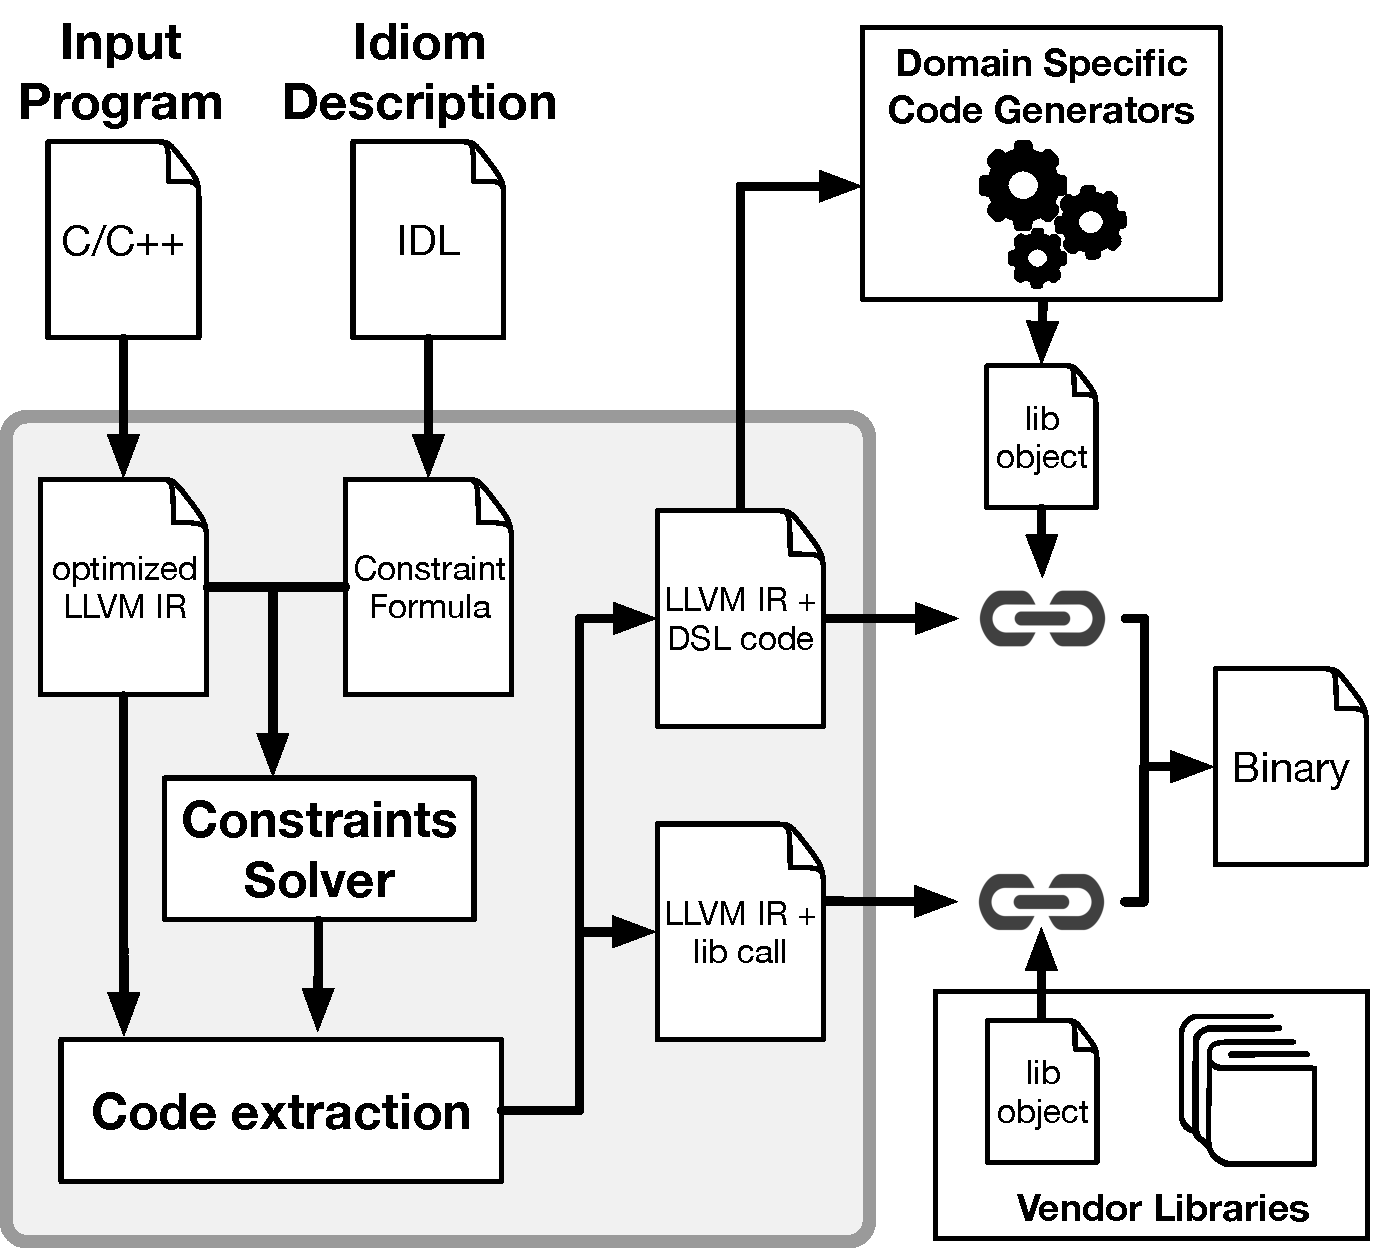
\includegraphics[width=\linewidth]{figures/compiler_flow.pdf}
    \caption{Workflow of our system}
    \label{fig:methodology}
    \vspace{-0.5em}
\end{figure}

    The program source code is compiled to optimised LLVM intermediate
    representation code and the idiom description is translated into constraints
    and represented internally as a C++ object.
    The C++ representation of the constraints and the user program LLVM IR code
    are then passed as inputs to a backtracking solver
    \cite{ginsbach2017discovery}, which detects all cases where the idioms can
    be found in the LLVR IR.

    The recognized idioms and the LLVM IR code are then passed on
    to the transformation phase of our system.
    The sections of code corresponding to computational idioms are extracted
    and reformulated for the appropriate heterogeneous APIs.
    For libraries this means replacing
    the code covered by the idiom with a library call. 
    For domain specific language interfaces,
    things are a little more involved. As before, we first extract the code
    associated with the idiom and replace it with a function call. This
    extracted code is now translated into the appropriate DSL and then
    passed on to the external DSL compiler which optimizes and generates
    code. The generated code is then linked
    with the object code from the main program.

    Determining the best heterogeneous APIs to use for a given platform
    and the best idioms to exploit will become a major issue as the number
    of idioms and APIs grows.  Currently, in this paper, we just try all
    applicable libraries and DSLs and pick the best executing
    code. Determining the best option is future work.

\begin{figure}[p]
    \begin{lstlisting}[language=MyCpp, basicstyle=\linespread{0.75}\small\ttfamily]
for (j = 0; j < ([{\bf m}]); j++) {
  d = 0.0;
  for (k = ([{\bf rowstr }])[j]; k < ([{\bf rowstr}])[j+1]; k++)
    d = d + ([{\bf a}])[k]*([{\bf z}])[([{\bf colidx}])[k]];
  ([{\bf r}])[j] = d; }
\end{lstlisting}
\vspace{-4.4mm}
\begin{lstlisting}[language={LLVM}, basicstyle=\linespread{0.75}\tiny\ttfamily,
                   label={fig:spmvexample1}, caption={Sparse linear algebra in C and LLVM IR}]
; <label>:2:
  %j = phi i64 [ %j_next, %12 ], [ 0, %1 ]
  %j_cond = icmp slt i64 %j, ([{\bf \%m}])
  br i1 %j_cond, label %3, label %13([\vspace{1mm}])
; <label>:3:
%4 = getelementptr i32, i32* ([{\bf \%rowstr}]), i64 %j
  %5 = load i32, i32* %4
  %j_next = add nuw nsw i64 %j, 1
  %6 = getelementptr i32, i32* ([{\bf \%rowstr}]), i64 %j_next
  %7 = load i32, i32* %6
  %k_begin = sext i32 %5 to i64
  %k_end = sext i32 %7 to i64
  br label %8([\vspace{1mm}])
; <label>:8:
  %k = phi i64 [ %k_next, %9 ], [ %k_begin, %dnext ]
  %d = phi double [ 0.0, %3 ], [ %d_next, %9 ]
  %k_cond = icmp slt i64 %iv, %k_end
  br i1 %k_cond, label %9, label %12([\vspace{1mm}])
; <label>:9:
  %a_addr = getelementptr double, double* ([{\bf \%a}]), i64 %k
  %a_load = load double, double* %a_addr
  %cix_addr = getelementptr i32, i32* ([{\bf \%colidx}]), i64 %k
  %cix_load = load i32, i32* %cix_addr
  %10 = sext i32 %cix_load to i64
  %z_addr = getelementptr double, double* ([{\bf \%z}]), i64 %10
  %z_load = load double, double* %z_addr
  %11 = fmul double %a_load, %z_load
  %d_next = fadd double %d, %11
  %k_next = add nsw i64 %k, 1
  br label %8([\vspace{1mm}])
; <label>:12:
  %r_addr = getelementptr double, double* ([{\bf \%r}]), i64 %j
  store double %d, double* %r_addr
  br label %2
\end{lstlisting}
\vspace{-0.287cm}
%\end{figure}

\centering
\vspace{0.0em}
{\centering
\begin{minipage}{0.05\linewidth}
\vspace{0pt}
\centering
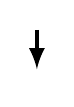
\begin{tikzpicture}[ultra thick]
 \draw [black,   -latex      ] (0,0.5) -- (0,0) node [] {};
\end{tikzpicture}
\end{minipage}
\begin{minipage}{\linewidth}
% \vspace{-5pt}
\centering
\textbf{Idiom detection with IDL program in \Cref{fig:spmv}}
\end{minipage}
\begin{minipage}{0.05\linewidth}
\vspace{0pt}
\centering
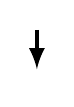
\begin{tikzpicture}[ultra thick]
 \draw [black,   -latex      ] (0,0.5) -- (0,0) node [] {};
\end{tikzpicture}
\end{minipage}
}

%\begin{figure}
{\centering
\footnotesize 
\begin{tabular}{l|l}
\textbf{Variable Name} & \textbf{Assigned IR Value}\\
\hline
iterator                    & \texttt{\%j}\\
inner.iter\_begin           & \texttt{\%k\_begin}\\
inner.iter\_end             & \texttt{\%k\_end}\\
inner.iterator              & \texttt{\%k}\\
idx\_read.value             & \texttt{\%cix\_load}\\
indir\_read.value           & \texttt{\%a\_load}\\
seq\_read.value             & \texttt{\%z}\\
\end{tabular}
\hspace{0.5cm}
\begin{tabular}{l|l}
\textbf{Variable Name} & \textbf{Assigned IR Value}\\
\hline
output.address              & \texttt{\%r\_addr}\\
iter\_begin                 & \texttt{0}\\
iter\_end                   & \texttt{\%\bf m}\\
idx\_read.base\_pointer     & \texttt{\%\bf colidx}\\
seq\_read.base\_pointer     & \texttt{\%\bf a}\\
indir\_read.base\_pointer   & \texttt{\%\bf z}\\
\dots                       & \dots\vspace{-0.5mm}\\
\end{tabular}

}

\caption{Constraint solution for sparse mv}
\label{fig:spmvexample2}
%\end{figure}

\centering
\vspace{0.0em}
{\centering
\begin{minipage}{0.05\linewidth}
\vspace{0pt}
\centering
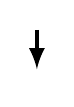
\begin{tikzpicture}[ultra thick]
 \draw [black,   -latex      ] (0,0.5) -- (0,0) node [] {};
\end{tikzpicture}
\end{minipage}
\begin{minipage}{\linewidth}
% \vspace{-5pt}
\centering
\textbf{Code generation: insert arguments, replace code}
\end{minipage}
\begin{minipage}{0.05\linewidth}
\vspace{0pt}
\centering
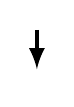
\begin{tikzpicture}[ultra thick]
 \draw [black,   -latex      ] (0,0.5) -- (0,0) node [] {};
\end{tikzpicture}
\end{minipage}
}


%\begin{figure}
\begin{lstlisting}[language=C, basicstyle=\linespread{0.75}\small\ttfamily,
                   label={fig:spmvexample3}, caption={Generated function call to cuSPARSE}]
cusparseDcsrmv(context,
    CUSPARSE_OPERATION_NON_TRANSPOSE, ([{\bf m}]), n,
    ([{\bf rowstr}])[([{\bf m}])+1]-([{\bf rowstr}])[0], &gpu_1, descr, gpu_([{\bf a}]),
    gpu_([{\bf rowstr}]), gpu_([{\bf colidx}]), gpu_([{\bf z}]), &gpu_0, gpu_([{\bf r}]));
\end{lstlisting}
\vspace{-0.287cm}
\end{figure}

\subsection{Sparse Linear Algebra in IDL}

    Although the previous example illustrated how constraints can be applied to 
    program analysis, we want to detect much more complex idioms and 
    map them to existing APIs.

    The code in \Cref{fig:spmvexample1} shows the performance bottleneck of
    the NAS \emph{Conjugate Gradient (GC)} benchmark, as well as the
    corresponding LLVM IR code.
    It implements a standard operation from sparse linear algebra, namely a
    multiplication of a sparse matrix in Compressed Sparse Row (CSR) format with
    a dense vector.

    This code contains several features that make it unsuitable for most
    established compiler optimizations:
    The iteration domain of the nested loop is memory dependent (line 3) and
    there is indirect memory access (line 4).
    This makes the iteration domain of the loop nest non-polyhedral and the
    access structure to memory non-affine.
    Under these conditions, simple data dependence models, but also
    sophisticated analysis based on the polyhedral model, would fail.

    We can express this idiom in IDL (\Cref{sec:idioms}, \Cref{fig:spmv}).
    The IR code, together with the IDL program, is fed into a constraint solver,
    which outputs a constraint solution as shown in \Cref{fig:spmvexample2}.
    We can see that different parts of the IR have been assigned to IDL
    variables.

    \Cref{fig:spmvexample3} shows how this solution is used to generate a
    call to a cuSPARSE procedure.
    The individual solution variables are inserted into the {\tt cusparseDcsrmv}
    code template as function arguments. 
    The original code is then cut out and replaced with this function call.
    The cuSPARSE library is then linked with the object code produced by the
    LLVM compiler, resulting in a speedup of $17\times$ on a GPU as described in
    \Cref{sec:idiomresults}.

    Central to our approach is the ability to detect idioms.
    In the next section we introduce a powerful description language that is
    capable of expressing a wide class of idioms that are suitable for
    acceleration by heterogeneous hardware.

\newpage

\section{Specification of Idioms in IDL}
\label{sec:idioms}

    The specification of computational idioms in IDL requires a careful
    handling of the arising complexity, using the modularity functionality that
    IDL provides.

    Control flow constructs, memory access patters as well as basic data flow
    patterns are specified independently and then combined together in order to
    define the complete constraint specifications.


\begin{figure}[p]
\begin{lstlisting}[language={constraints},numbers=none,xleftmargin=0cm,framexleftmargin=0em,basicstyle=\linespread{1.133}\scriptsize\ttfamily]
Constraint SESE
( {precursor} is branch instruction and
  {precursor} has control flow to {begin} and
  {end} is branch instruction and
  {end} has control flow to {successor} and
  {begin} control flow dominates {end} and
  {end} control flow post dominates {begin} and
  {precursor} strictly control flow dominates
      {begin} and
  {successor} strictly control flow post dominates
      {end} and
  all control flow from {begin} to {precursor}
      passes through {end} and
  all control flow from {successor} to {end}
      passes through {begin})
End
\end{lstlisting}
\vspace{-.3cm}
\caption{IDL specification of SESE region\vspace{-.3em}}
\label{fig:sese}
\end{figure}

\begin{figure}[p]
\vspace{.512cm}
\begin{lstlisting}[language={constraints},numbers=none,xleftmargin=0cm,framexleftmargin=0em,basicstyle=\linespread{1.133}\scriptsize\ttfamily]
Constraint GEMM
( inherits ForNest(N=3) and
  inherits MatrixStore
      with {iterator[0]} as {col}
       and {iterator[1]} as {row}
       and {begin} as {begin} at {output} and
  inherits MatrixRead
      with {iterator[0]} as {col}
       and {iterator[2]} as {row}
       and {begin} as {begin} at {input1} and
  inherits MatrixRead
      with {iterator[1]} as {col}
       and {iterator[2]} as {row}
       and {begin} as {begin} at {input2} and
  inherits DotProductLoop
      with {loop[2]}        as {loop}
       and {input1.value}   as {src1}
       and {input2.value}   as {src2}
       and {output.address} as {update_address})
End
\end{lstlisting}
\vspace{-.3cm}
\caption{IDL specification of GEMM}
\label{fig:gemm}
\vspace{.512cm}
\end{figure}

\begin{figure}[p]
\begin{lstlisting}[language={constraints},numbers=none,xleftmargin=0cm,framexleftmargin=0em,basicstyle=\linespread{1.133}\scriptsize\ttfamily]
Constraint Histogram
( inherits For and
  inherits ConditionalReadModifyWrite
      with {indexkernel.output} as {address}
       and {kernel.output} as {value} and
  collect i
  ( inherits VectorRead
        with {read_value[i]} as {value}
         and {iterator} as {idx}
         and {begin} as {begin} at {read[i]}) and
  inherits Concat
      with {read_value}   as {in1}
       and {old_value}    as {in2}
       and {kernel.input} as {out} and
  inherits KernelFunction
      with {begin} as {outer}
       and {body.begin} as {inner} at {kernel} and
  inherits KernelFunction
      with {read_value} as {input}
       and {begin} as {outer}
       and {body.begin} as {inner} at {indexkernel})
End
\end{lstlisting}
\vspace{-.3cm}
\caption{IDL specification of generalized histogram}
\label{fig:histogram}
\end{figure}

\begin{figure}[p]
\begin{lstlisting}[language={constraints},numbers=none,xleftmargin=0cm,framexleftmargin=0em,basicstyle=\linespread{1.133}\scriptsize\ttfamily]
Constraint SPMV
( inherits For and
  inherits VectorStore
      with {iterator} as {idx}
       and {begin} as {begin} at {output} and
  inherits ReadRange
      with {iterator} as {idx} 
       and {inner.iter_begin} as {range_begin} 
       and {inner.iter_end}   as {range_end} and
  inherits For at {inner} and
  inherits VectorRead
      with {inner.iterator} as {idx}
       and {begin} as {begin} at {idx_read} and
  inherits VectorRead
      with {idx_read.value} as {idx}
       and {begin} as {begin} at {indir_read} and
  inherits VectorRead
      with {inner.iterator} as {idx}
       and {begin} as {begin} at {seq_read} and
  inherits DotProductLoop
      with {inner}            as {loop}
       and {indir_read.value} as {src1}
       and {seq_read.value}   as {src2}
       and {output.address}   as {update_address})
End
\end{lstlisting}
\vspace{-.3cm}
\caption{IDL specification of SPMV}
\label{fig:spmv}
\vspace{.3cm}
\end{figure}

\begin{figure}[p]
\begin{lstlisting}[language={constraints},numbers=none,xleftmargin=0cm,framexleftmargin=0em,basicstyle=\linespread{1.133}\scriptsize\ttfamily]
Constraint Stencil
( inherits ForNest and
  inherits PermMultidStore
      with {iterator} as {input} 
       and {begin} as {begin} at {write} and
  collect i
  ( inherits StencilRead
      with {write.input_index} as {input}
       and {kernel.input[i]} as {value}
       and {begin} as {begin} at {reads[i]}) and
  {kernel.output} is first argument of {write.store} and
  inherits KernelFunction
      with {begin}      as {outer}
       and {body.begin} as {inner} at {kernel})
End
\end{lstlisting}
\vspace{-.3cm}
\caption{IDL specification of simple stencil}
\label{fig:stencilcompute}
\vspace{.3cm}
\end{figure}

\begin{figure}[p]
\begin{lstlisting}[language={constraints},numbers=none,xleftmargin=0cm,framexleftmargin=0em,basicstyle=\linespread{1.133}\scriptsize\ttfamily]
Constraint Reduction
( inherits For and
  collect i
  ( inherits VectorRead
        with {iterator}         as {idx}
         and {read_value[i]}    as {value}
         and {begin} as {begin} at {read[i]}) and
  inherits InductionVar
       with {old_value}       as {old_ind}
        and {kernel.output}   as {new_ind} and
  {old_value} is not the same as {iterator} and
  inherits Concat
      with {read_value}   as {in1}
       and {old_value}    as {in2}
       and {kernel.input} as {out} and
  inherits KernelFunction
      with {begin}      as {outer}
       and {body.begin} as {inner} at {kernel})
End
\end{lstlisting}
\vspace{-.3cm}
\caption{IDL specification of scalar reductions}
\label{fig:scalarreduction}
\end{figure}

\subsection{Dense Linear Algebra}

    The generalized matrix multiplication idiom is described in \Cref{fig:gemm}.
    The control flow is captured by three nested for loops.
    Inside these loops, the memory access is characterized by three matrix
    accesses, each with a different subset of the loop iterators.
    The corresponding \texttt{MatrixRead} and \texttt{MatrixWrite} idioms model
    generic access to matrices allowing strides, transposed matrices etc.
    The actual computation is encapsulated by the \texttt{DotProductLoop} idiom.
    This also contains the linear combination with factors \texttt{alpha} and
    \texttt{beta} that is part of the generalized matrix multiplication.

    The sparse matrix vector multiplication defined in \Cref{fig:spmv} is
    different to the other idioms in that
    the control flow of the skeleton of the idiom does not consist of perfectly
    nested for loops.
    Instead, the iteration space of the inner loop is read from an array using
    the \texttt{ReadRange} idiom.
    The actual computation that SPMV performs is a dot product and thus it uses
    the same \texttt{DotProductLoop} idiom as
    \texttt{GEMM} but the memory access pattern is different, with indirect
    memory access in \texttt{indir\_read}.

\subsection{Sparse Linear Algebra}
At the heart of our approach is a simple language to specify sparse and dense
linear algebra operations.
This serves two purposes in our LiLAC system: Firstly, it is used to generate
a detection program for finding the computation in user code.
Secondly, it identifies the variables that are arguments to the library, thus
defining the harness interface.

The key challenge in the design of this language was to stay simple enough
to allow automatic generation of robust detection functionality, yet to be able
to capture interesting functionality.
Crucial for sparse linear algebra routines is capturing the many different
memory access patterns, the control flow on the other hand is very rigid.
This is reflected in the grammar as shown in \autoref{bnfgrammar}.

\subsection{Sparse Matrix Variations in LiLAC-What}
Sparse matrices can be stored in different formats.
In this section we introduce two of them and show how LiLAC-What can express
the corresponding computations.

\begin{figure}[t]
\begin{align*}
program ::=\ &\textbf{COMPUTATION} \left<name\right> \left<body\right>\\
body    ::=\ &\left<forall\right> \mid \left<dotop\right>\\
range   ::=\ &\textbf{(} \left<exp\right> \textbf{<=} \left<name\right> \textbf{<} \left<exp\right> \textbf{)}\\
forall ::=\ &\textbf{forall} \left<range\right> \textbf{\{} \left<body\right> \textbf{\}}\\
dotp    ::=\ &\left<addr\right> \textbf{=}\ \textbf{dot} \left<range\right> \left<addr\right> \textbf{*} \left<addr\right> \textbf{;}\\
addr    ::=\ &\left<name\right> \{\ \textbf{[} \left<exp\right> \textbf{]}\ \}\\
add     ::=\ &\left<exp\right> \textbf{+} \left<exp\right>\\
mul     ::=\ &\left<exp\right> \textbf{*} \left<exp\right>\\
exp     ::=\ &\left<name\right> \mid \left<cnst\right> \mid \left<addr\right> \mid\ \left<add\right> \mid \left<mul\right>
\end{align*}
\vspace{-1.5em}
\caption{Grammar of the LiLAC-What language}
\label{bnfgrammar}
\end{figure}

\begin{figure}[t]
\begin{minipage}[b]{0.3\linewidth}
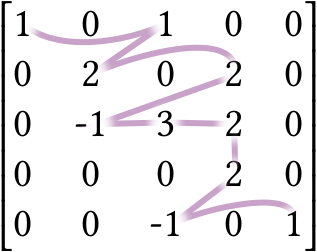
\includegraphics[width=0.9\linewidth]{figures/csrorder.png}
\vspace{0.04em}
\end{minipage}
\begin{minipage}[b]{0.65\linewidth}
\begin{align*}
\text{\bf val} =& \begin{bmatrix}
1\ \ 1\ \ 2\ \ 2\ \ \text{-}1\ \ 3\ \ 2\ \ 2\ \ \text{-}1\ \ 1\\
\end{bmatrix}\\
\text{\bf col\_ind} =& \begin{bmatrix}
0\ \ 2\ \ 1\ \ 3\ \ 1\ \ 2\ \ 3\ \ 3\ \ 2\ \ 4\\
\end{bmatrix}\\
\text{\bf row\_ptr} =& \begin{bmatrix}
0\ \ 2\ \ 4\ \ 7\ \ 8\ \ 10\\
\end{bmatrix}
\end{align*}
\end{minipage}
\vspace{0.5em}
\hrule
\vspace{0.3em}
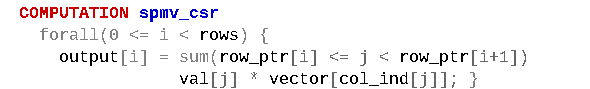
\includegraphics[width=\linewidth]{figures/spmvcsrwhat.pdf}
\vspace{-1.2em}
\caption{Compressed Sparse Row in LiLAC-What}
\label{csr_lilacwhat_fig}
\vspace{1.5em}
\centering
\begin{minipage}[b]{0.3\linewidth}
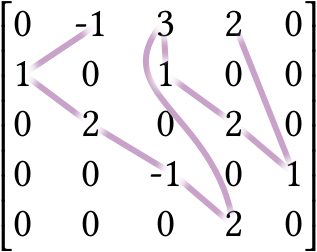
\includegraphics[width=0.9\linewidth]{figures/jdsorder.png}
\vspace{0.04em}
\end{minipage}
\begin{minipage}[b]{0.65\linewidth}
\footnotesize
\begin{align*}
\text{\bf perm} =& \begin{bmatrix}1\ \ 2\ \ 0\ \ 4\ \ 3\\\end{bmatrix}\\[-0.4em]
\text{\bf val} =& \begin{bmatrix}\text{-}1\ \ 1\ \ 2\ \ \text{-}1\ \ 2\ \ 3\ \ 1\ \ 2\ \ 1\ \ 2\\\end{bmatrix}\\[-0.4em]
\text{\bf col\_ind} =& \begin{bmatrix}1\ \ 0\ \ 1\ \ 2\ \ 3\ \ 2\ \ 2\ \ 3\ \ 4\ \ 3\\\end{bmatrix}\\[-0.4em]
\text{\bf jd\_ptr} =& \begin{bmatrix}0\ \ 5\ \ 9\ \ 10\\\end{bmatrix}\\[-0.4em]
\text{\bf nzcnt} =& \begin{bmatrix}3\ \ 2\ \ 2\ \ 2\ \ 1\end{bmatrix}
\end{align*}
\end{minipage}
\vspace{0.5em}
\hrule
\vspace{0.3em}
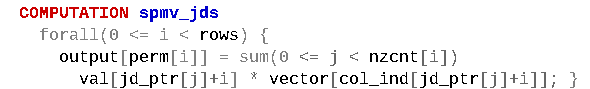
\includegraphics[width=\linewidth]{figures/spmvjdswhat.pdf}
\vspace{-1.2em}
\caption{Jagged Diagonal Storage in LiLAC-What}
\label{jds_lilacwhat_fig}
\end{figure}

\subsubsection{Compressed Sparse Row}
For Compressed Sparse Row (CSR) \cite{doi:10.1137/1.9780898718003}, all non-zero
entries are stored in a flat array \textbf{val}.
The \textbf{col\_ind} array stores the column position for each value.
Finally, the \textbf{row\_ptr} array stores the beginning of each row of the
matrix as an offset into the other two arrays.
The number of rows in the matrix is given directly by the length of the
\textbf{row\_ptr} array minus one, however the number of columns is not
explicitly stored.
In \autoref{csr_lilacwhat_fig}, a 5x5 matrix is shown represented in this
format.

\subsubsection{Jagged Diagonal Storage}
For Jagged Diagonal Storage (JDS) \cite{doi:10.1137/0910073}, the rows of the
matrix are permuted such that the number of nonzeros  per row  decreases. The
permutation is stored in a vector \textbf{perm}, the number of nonzeros in
\textbf{nzcnt}.
The nonzero entries are then stored in an array \textbf{val} in the following
order: The first nonzero entry in each row, then the second nonzero entry in
each row etc.
The array \textbf{col\_ind} stores the column for each of the values and
\textbf{jd\_ptr} stores offsets into \textbf{val} and \textbf{col\_idx}.
The product of a sparse matrix in JDS format with a dense vector is specified 
in LiLAC-What at the bottom of \autoref{jds_lilacwhat_fig}.

\subsection{Stencils}
    \Cref{fig:stencilcompute} shows the basic stencil idiom.
    Stencils consist of a loop nest with a multi-dimensional memory access to
    store the updated cell value.
    This updated value is computed with a kernel function using a number of
    values that are constraint by the
    \texttt{StencilRead} idiom, which specifies multidimensional array access
    with only constant offsets in all dimensions.

\subsection{Not Syntactic Pattern Matching}
The idiom descriptions may at first appear to be shallow syntactic pattern matching.
In fact, because it operates on the IR level, it can detect idioms that are written in superficially distinct style but are semantically equivalent.
For example, there are two syntactically distinct programs in \Cref{fig:gemmexamples}, which in fact are both implementations of general matrix multiplication.
The IDL in \Cref{fig:gemm} discovers they are both instances of GEMM and they can both be replaced with an API call to GEMM.

\begin{figure}[ht]
\begin{lstlisting}[language=MyCpp]
for (int mm = 0; mm < m; ++mm) {
  for (int nn = 0; nn < n; ++nn) {
    float c = 0.0f;
    for (int i = 0; i < k; ++i) {
      float a = A[mm + i * lda]; 
      float b = B[nn + i * ldb];
      c += a * b;
    }
    C[mm+nn*ldc] =
        C[mm+nn*ldc] * beta + alpha * c;
  }
}
\end{lstlisting}
\begin{lstlisting}[language=MyCpp,label={fig:gemmexamples},caption=
   {Two matching instances of GEMM}]
for(int i = 0; i < 1000; i++)
    for(int j = 0; j < 1000; j++) {
        M3[i][j] = 0.0f;
        for(int k = 0; k < 1000; k++)
           M3[i][j]+=M1[i][k]*M2[k][j]; }
\end{lstlisting}
\end{figure}

    There are limitations to this semantic matching.
    In particular, the use of low level manual optimizations that circumvent the
    usual IR representation, {\em e.g.}  SIMD compiler intrinsics, would distort
    the algorithms beyond recognition by our system.
    In practice, this is rarely encountered.

\subsection{Compilation Process and Implementation}
\label{sec:compilation}

    Idiom definitions are compiled to C++ functions that perform idiom
    recognition on LLVM IR.
    In a first step, the compiler eliminates
    $\left<\text{\tt inheritance}\right>$, $\left<\text{\tt forall}\right>$,
    $\left<\text{\tt forsome}\right>$, $\left<\text{\tt if}\right>$,
    $\left<\text{\tt rename}\right>$ and $\left<\text{\tt rebase}\right>$.
    They are replaced with simpler $\left<\text{\tt conjunction}\right>$ and
    $\left<\text{\tt disjunction}\right>$ constructs.
    This also involves removing all parameterizations from the formula and
    flattening all variable names.
    Next, variables are collected and ordered to assist constraint solving.
    The ordering impacts performance, as it determines how well the search space
    is pruned. 
    For each variable, all the constraints associated with the variable are
    assembled.

    The compiler then emits C++ code which is passed to a generic solver based on \cite{ginsbach2017discovery} to search for idiom instances.
    This solver is based on standard backtracking.
    As shown in the results section, this increases compilation time, but the overhead is modest.

\section{Targeted Heterogeneous APIs}

    After idiom detection, we must transform the user program to exploit the
    relevant API.
    Two types of heterogeneous APIs are currently targeted: libraries and domain
    specific languages with their optimizing compilers.

    \subsection{Domain Specific Libraries}
    Libraries provide narrow interfaces but are often highly optimised.
    For example, the cuBLAS library is only suitable for a limited set of dense
    linear algebra operations and only works on Nvidia GPUs, but its
    implementation provides outstanding performance.
    For sparse linear algebra we use the vendor provided cuSPARSE, clSPARSE, and
    MKL libraries.
    For dense BLAS routines cuBLAS, clBLAS, CLBlast, and MKL are used.

    \subsection{Domain Specific Code Generators}
    Domain Specific Languages provide wider interfaces than libraries and allow
    problems to be expressed as composition of dedicated language constructs.
    An optimizing compiler then specializes the program for the target hardware.
    We currently support Halide and Lift as domain specific code generators.

    \paragraph*{Halide}~\cite{Ragan-Kelley2013Halide} is a language and
    optimizing compiler targeted at image processing applications.
    Optimised code is generated for CPUs as well as GPUs.
    Halide separates the functional description of the problem from the
    description of the implementation which is called a \emph{schedule}.
    This allows retargeting of Halide programs to different platforms.
    We translate some of the stencil idioms and linear algebra idioms into
    Halide.
    Stencils involving control flow in their computations are not easily
    expressible in Halide.

    \paragraph*{Lift}~\cite{steuwer15rewrite, SteuwerRD17, HagedornSSGD18} is an
    optimizing code generator based on rewrite rules.
    The Lift language consists of functional parallel patterns such as
    \emph{map} and \emph{reduce} which  express a range of parallel
    applications.
    For this work we translate stencil idioms, complex reductions and linear
    algebra idioms to Lift.

\section{Translating Computational Idioms}

    This section describes how the detected idioms are mapped to the previously
    described library APIs domain specific languages.
    The two types of APIs (library interfaces and domain specific languages) are
    treated individually.

\subsection{Library}

    For library call interfaces, the original code is removed and an appropriate
    function call is inserted.
    The solution that is generated by the solver using the IDL program contains
    both the IR instructions to remove as well as the arguments that are to be
    used for the function call.

    For example, in the case of the {\tt GEMM} program that was shown in
    \Cref{fig:gemm}, the original code is removed by deleting the IR
    instruction at {\tt output.store\_instr} explicitly, which captures the
    store instruction of the {\tt MatrixStore} subprogram.
    The remaining cleanup is left to the standard dead code elimination pass.
    The arguments that specify the matrix dimensions are taken from
    {\tt ForNest} in combination with the stride and offset determined by
    {\tt MatrixRead} and {\tt MatrixWrite}.

    The mapping of solution variables to the arguments of the generated function
    call needs to be implemented individually for each backend, as we have no
    way to describe it in IDL itself.
    Once the code is replaced, LLVM continues with code generation as usual.

\subsection{DSL}

    For domain specific languages, the situation is a bit more involved.
    Reduction, histogram and stencil idioms are higher order functions that
    contain a kernel function or reduction operator that has to be represented
    for the DSL.

    For each combination of idiom and DSL there is a parameterized
    skeleton program.
    This skeleton is then specialized for the appropriate data types and numeric
    parameters as well as the kernel function or reduction operator.

    Numerical parameters are picked from the constraint solution in the same way
    that was described previously for library call interfaces.
    Also from the constraint solution, we have the loop body that contains the
    kernel function or reduction operator, as well as the input values and the
    result value used.
    We use this information to cut out the kernel function that is then used to
    generate code appropriate for the DSL backends:

\paragraph*{Lift}  expects stencil kernels or reduction operators to be sequential C code with a specific function interface that
is used internally by Lift when generating OpenCL code.
We therefore implemented a rudimentary LLVM IR to C backend for generating this function.

\paragraph*{Halide} is a language embedded in C++, it requires a syntax tree of the kernel functions built using a class hierarchy.

\begin{figure}[ht]
\begin{lstlisting}[language=LIFT,escapechar=|,
                   label={fig:liftmxm},caption=
   {Example of matrix multiplication in Lift}]
float mult(float x, float y) { return x*y; }
float add(float x, float y) { return x+y; }

gemm_in_lift(A, B, C, alpha, beta) {
 map(fun(a_row, c_row) {
  map(fun(b_col, c) {
   map(fun(ab){ add(mult(alpha, ab), mult(beta, c))},
    |\label{line:dot}|reduce(add, 0.0f, map(mult, zip(a_row, b_col))))
  }, zip(transpose(B), c_row))
 }, zip(A, C))
}
\end{lstlisting}
\end{figure}

\paragraph*{}
After code for the DSLs is generated, it is passed to the DSL code generator.
\Cref{fig:liftmxm} shows an example of the Lift code generated for GEMM (\texttt{gemm\_in\_lift}).
It performs a dot product (expressed in line~\ref{line:dot} using the Lift skeletons \texttt{zip}, \texttt{map}, and \texttt{reduce}) for each row of matrix A (\texttt{a\_row}) and column of matrix B (\texttt{b\_col}).
This code is compiled by Lift into optimised OpenCL code.

Finally, we again replace the idiom code in the user's code with a call to the code generated by the DSL and continue once again with LLVM code generation.

\subsection{Aliasing}

    Since idiom detection works statically, we are unable to fully rule out
    aliasing of pointers, which can make transformations unsound.
    For dense linear algebra this is easily solved with some basic run time
    checks for non-overlapping memory.
    However, for sparse linear algebra this is not as straightforward and in
    corner cases our approach is unsound.
    In practice this did not cause problems on any of the benchmark programs,
    however this means that optimizations based on these techniques will have to
    provide appropriate feedback to the programmer.

\section{Experimental Setup}

    \paragraph*{Benchmarks}
    We applied our approach to all of the sequential C/C++ versions of the NAS
    Parallel Benchmarks.
    We use the SNU NPB implementation by the Seoul National University,
    containing the original 8 NAS benchmarks plus two of the newer unstructured
    components UA and DC.
    We also evaluated our approach on all Parboil benchmarks, giving 21 programs
    in total. 

    \paragraph*{Platform and Evaluation}
    We use an AMD A10-7850K APU with a multi-core CPU and an integrated Radeon
    R7 GPU on the same die using driver version 1912.5, as well as an Nvidia GTX
    Titan X as an external GPU using driver version 375.66.
    We report the median runtime of 10 executions for each program.

    \paragraph*{Alternative detection approaches}
    \hspace{0.2cm}There are no easily available compilers to compare against
    that perform idiom detection.
    Instead, we consider two parallelizing compilers and examine
    whether they detect idioms as part of their parallelization approach.
    As their goal is parallelization and not idiom detection, this should be
    borne in mind in the results section.

    Polly \cite{Doerfert2015Polly} is an LLVM based polyhedral compiler
    capable of finding parallel loops and reductions in Static Control
    Parts (SCoP) of programs.  This allows comparison against
    another approach that uses the same compiler infrastructure.
    We gathered the SCoPs that Polly detected with the options
    \texttt{-O3 -mllvm -polly -mllvm -polly-export} and manually inspected
    the reported SCoPs for stencil like parallel loops and reduction operations.
    When Polly captured such a loop as a SCoP, we counted it as an idiom
    detection, although Polly itself has no concept of idioms.
    This gives an optimistic estimate as to what idiom coverage a polyhedral
    based approach can achieve.

    The Intel C++ Compiler (ICC) is a mature industry strength compiler that
    provides a detection mechanism for parallelizing reduction idioms based on
    data dependency analysis.
    We use the \texttt{-parallel -qopt-report} command line options and checked
    in the optimization report files whether the corresponding loop is
    considered parallelizable.

\newpage
\phantom{placeholder}
\newpage

\section{Results}
\label{sec:idiomresults}

    The approach was evaluated in several steps.
    Firstly, the number of detected idioms and their distribution over the
    benchmark programs was established.
    During this analysis, the run time of the IDL-enabled Clang compiler was
    measured, and the compile time overhead of the solver over standard
    compilation evaluated.
    Next, the run time coverage of the idioms was determined for each
    benchmark program, to see where exploitation might be beneficial.

    Where runtime coverage was substantial, we report speedups over sequential C
    code and compare the performance of each of the targets APIs.
    We also compare against the handwritten OpenMP and OpenCL implementations
    that are included with the benchmark suites as reference implementations.

\begin{figure}[t]
  \centering
  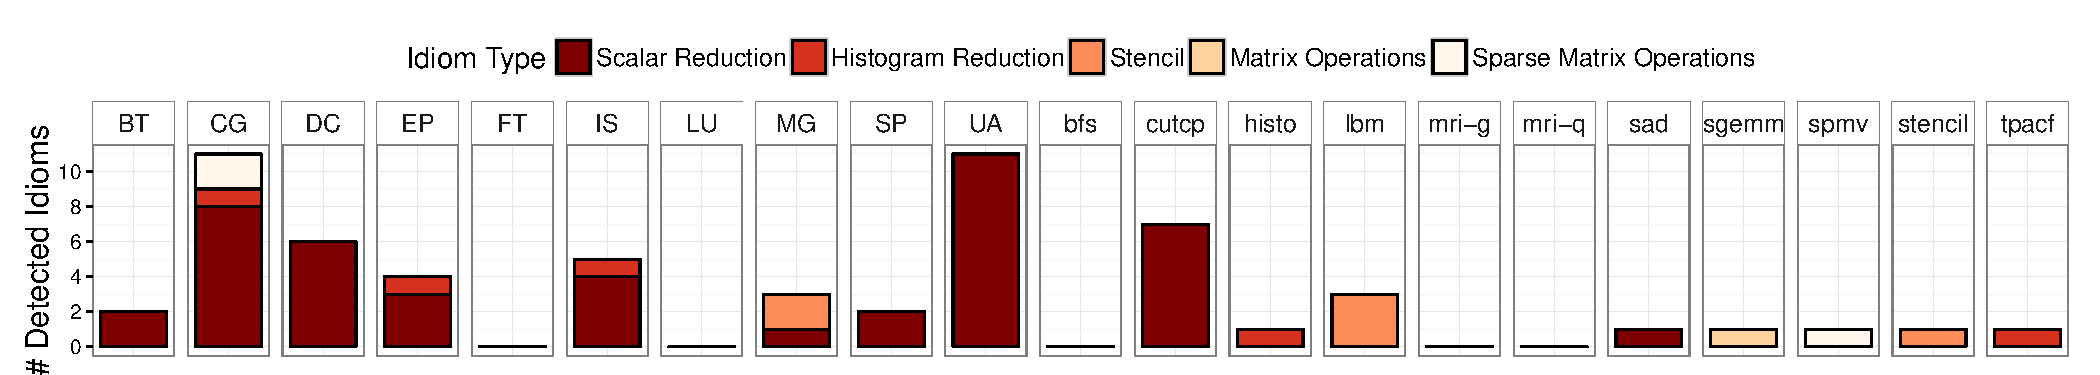
\includegraphics[width=\textwidth]{figures/asplosplots/detection.pdf}
  \caption{The different computational idioms found in all benchmarks.}
  \label{detection-figure}
\end{figure}
\begin{figure}[t]
  \centering
  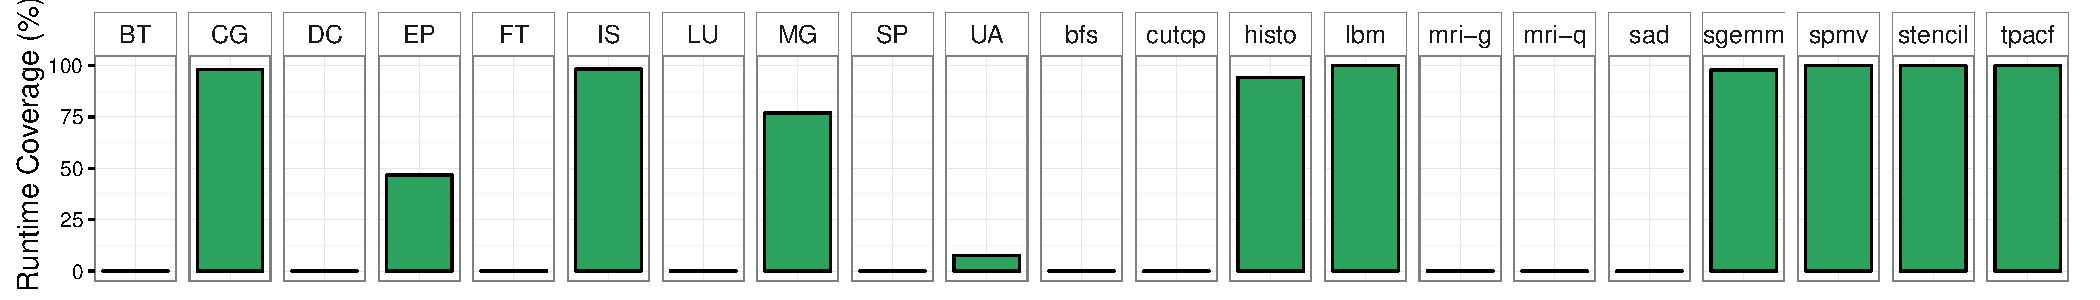
\includegraphics[width=\textwidth]{figures/asplosplots/coverage.pdf}
  \caption{Runtime coverage of the detected idioms in all benchmarks.}
  \label{coverage-figure}
  \vspace{0.5em}
\end{figure}

\subsection{Idiom Detection}

    \Cref{tab:detection} shows the number of idioms found by our approach, Polly, and ICC.
    Polly finds 3 scalar reductions and 6 stencils while ICC which just considers  scalar reduction finds 28.
    Polly is unable to perform idiom specific optimizations on GEMM.
    Other approaches do not detect any histograms or sparse matrix operations, because such code involves indirect and thus non-affine memory accesses.
    This fundamentally contradicts assumptions that these tools rely on and is not merely an implementation artifact.
    Our IDL approach detects 60 idioms overall with the compile time cost shown in figure \Cref{tab:compiletimecost}.
    On average, the compilation time is increased by 82\%, which can be reduced further by optimizing the solver.

    \Cref{detection-figure} shows the different idioms detected across
    the  benchmarks. We detect both scalar
    and histogram reductions as well as stencils, dense matrix operations
    and sparse matrix-vector multiplication.
    Polly and ICC are only capable of detecting simple scalar
    reductions, but we are able to detect histogram reductions, {\em e.g.} in
    the \emph{histo} benchmark as well.  For stencils, Polly detects two
    in \emph{lbm} and \emph{stencil} while our approach
    detects all the stencils in \emph{lbm}, \emph{stencil} and \emph{MG}.
    Unlike any existing approach, we detect sparse matrix-vector
    operations in {\emph CG} and {\emph spmv} as well as dense matrix
    operations in \emph{sgemm}. It is worth repeating, however, that both
    Polly and ICC are parallelizing compilers, not idiom recognition
    tools.

\begin{table}[t]
\centering
  \begin{tabular}{lP{2.16cm}P{2.16cm}P{2.16cm}P{2.163cm}P{2.163cm}}
  \toprule
  \hspace{1.18cm} & Scalar\newline{}Reduction & Histogram\newline{}Reduction & Stencil & Matrix~Op. & Sparse\newline{}Matrix~Op.\\
  \midrule
  Polly &  3  &  --- &   5  &  --- & --- \\
  ICC   &  28 &  --- &  --- &  --- & --- \\
  IDL   &  45 &   5  &   6  &   1  &  3  \\
  \bottomrule
\end{tabular}
\caption{Idioms detected by IDL, ICC, Polly}
\label{tab:detection}
\end{table}

\subsection{Runtime Coverage}

    To determine if the detected idioms are actually important,
    \Cref{coverage-figure} shows the percentage of time spent in the detected
    computational idiom.
    This data shows that either the detected idioms have a low runtime
    contribution or they dominate almost the entire execution.
    \emph{EP} is the only exception where about 50\% of the runtime is spent
    inside a detected histogram reduction.
    We focus on the 10 programs which spend a significant amount of time in the
    detected idioms, as only these can reasonably expect a performance gain
    using our approach.

\subsection{Performance Results}

\begin{table}[t]
\centering
\begin{tabular}{lcccccccccccc}
  \toprule
  & \hspace{0.17mm}BT\hspace{0.17mm}
  & \hspace{0.17mm}CG\hspace{0.17mm}
  & \hspace{0.17mm}DC\hspace{0.17mm}
  & \hspace{0.17mm}EP\hspace{0.17mm}
  & \hspace{0.17mm}FT\hspace{0.17mm}
  & \hspace{0.17mm}IS\hspace{0.17mm}
  & \hspace{0.17mm}LU\hspace{0.17mm}
  & \hspace{0.17mm}MG\hspace{0.17mm}
  & \hspace{0.17mm}SP\hspace{0.17mm}
  & \hspace{0.17mm}UA\hspace{0.17mm}
  & \hspace{0.17mm}bfs\hspace{0.17mm}
  & \hspace{0.17mm}cutcp\hspace{0.17mm} \\
  \midrule
without IDL    & 1.9 & 0.5 & 1.0 & 0.3 & 0.6 & 0.3 & 1.9 & 0.8 & 1.6 & 2.7 & 0.4 & 0.4 \\[0.25em]
with IDL       & 4.0 & 0.8 & 1.6 & 0.6 & 1.2 & 0.5 & 3.9 & 4.5 & 3.2 & 7.3 & 0.5 & 0.6 \\[0.75em]
overhead in \% & 116 &  77 &  57 &  77 &  93 &  62 & 103 & 484 &  97 & 169 &  30 &  65 \\
  \bottomrule
\end{tabular}
\vspace{5mm}

\begin{tabular}{lccccccccc}
  \toprule
  & \hspace{0.44mm}histo\hspace{0.44mm}
  & \hspace{0.44mm}lbm\hspace{0.44mm}
  & \hspace{0.44mm}mri-g\hspace{0.44mm}
  & \hspace{0.44mm}mri-q\hspace{0.44mm}
  & \hspace{0.44mm}sad\hspace{0.44mm}
  & \hspace{0.44mm}sgemm\hspace{0.44mm}
  & \hspace{0.44mm}spmv\hspace{0.44mm}
  & \hspace{0.44mm}stencil\hspace{0.44mm}
  & \hspace{0.44mm}tpacf\hspace{0.44mm} \\
  \midrule
without IDL    & 0.2 & 0.3 & 0.2 & 0.2 & 0.4 & 0.6 & 0.3 & 0.2 & 0.2 \\[0.25em]
with IDL       & 0.2 & 0.6 & 0.4 & 0.3 & 0.6 & 0.7 & 0.7 & 0.2 & 0.4 \\[0.75em]
overhead in \% &  35 &  87 & 100 &  52 &  58 &  24 & 115 &  36 &  54 \\
  \bottomrule
\end{tabular}
\caption{Compile time cost in seconds}
\label{tab:compiletimecost}
\end{table}

\paragraph*{Speedup vs. Sequential}
\Cref{fig:speedup-figure} shows the end-to-end speedup obtained by accelerating idioms with heterogeneous APIs on a CPU, an integrated GPU, and an external GPU.
All results include data transfer overhead to and from the GPUs.
Here the best performing API is shown;
\Cref{tab:detailed-results} provides detailed results for all APIs. 

\begin{figure}[t]
  \centering
  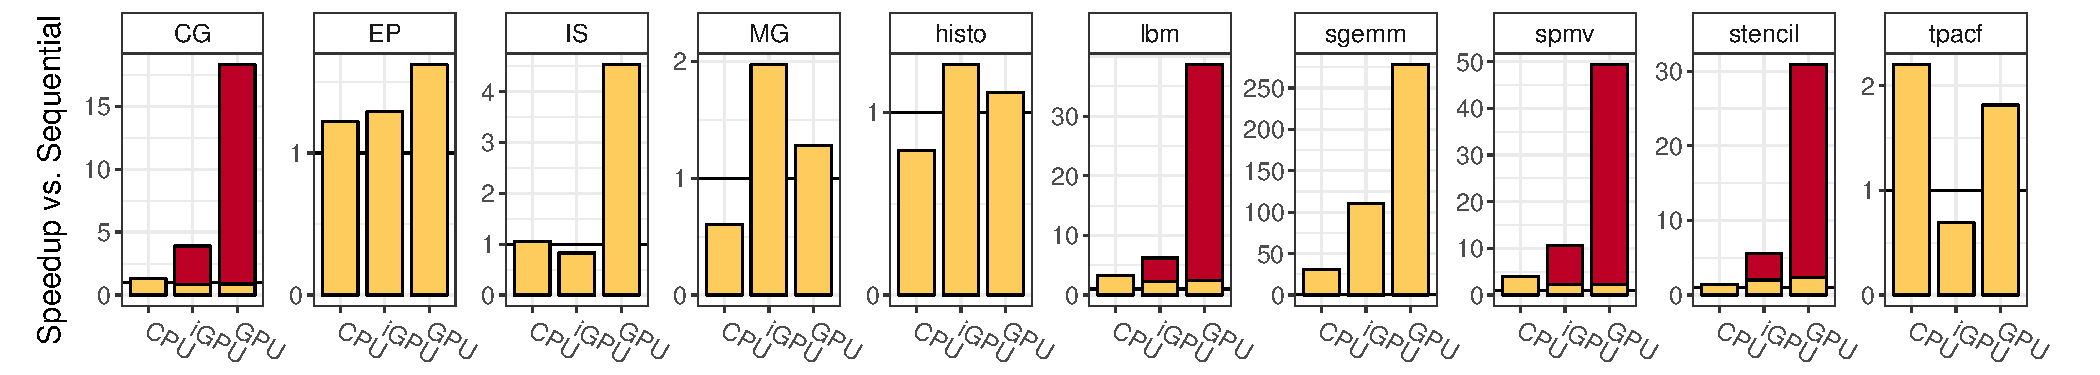
\includegraphics[width=\textwidth]{figures/asplosplots/speedup_vs_sequential_wide.pdf}
  \caption{Speedup compared to the sequential C program.
           Results for the best performing heterogeneous API on each device are shown.
           The red bars indicate a manual runtime optimization for avoiding unnecessary data transfers.}
  \label{fig:speedup-figure}
  \vspace{1.5em}
  \centering
  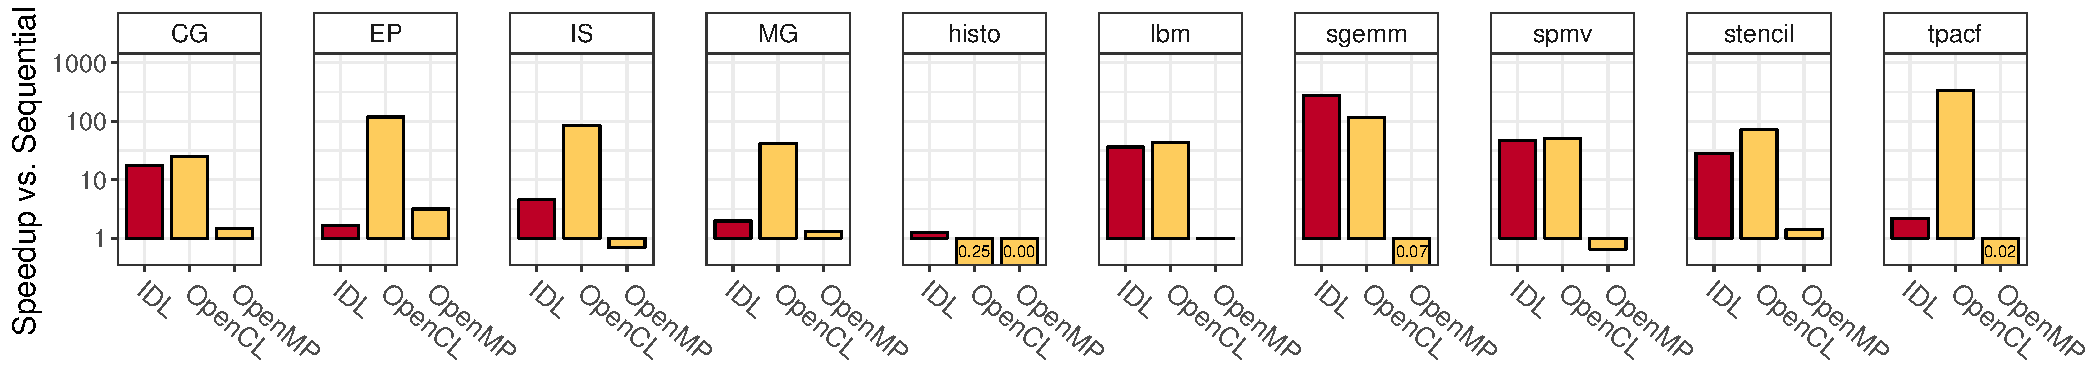
\includegraphics[width=\textwidth]{figures/asplosplots/comparison.pdf}
  \caption{Speedup of our constraints based approach (executed on the best hardware and highlighted in red) compared to handwritten parallel OpenCL (executed on the GPU) and OpenMP (executed on the CPU) implementations.}
  \label{fig:speedup-figure-2}
  \vspace{0.5em}
\end{figure}

\begin{landscape}
\newlength{\txtwd}
\newcommand{\msb}[1]{\settowidth{\txtwd}{#1}{\tiny\ttfamily\bfseries \hfill #1}}
\newcommand{\ms}[1]{\settowidth{\txtwd}{#1}{\tiny\ttfamily \hfill #1}}
\addtolength{\tabcolsep}{-0.64mm}
\begin{table}[p]
  \centering
  \small
  \begin{tabular}{|l||cccccc|ccccc|cccc|}
  \hline
  & \multicolumn{6}{c|}{\bfseries\large CPU} & \multicolumn{5}{c|}{\bfseries\large iGPU} & \multicolumn{4}{c|}{\bfseries\large GPU} \\[3mm]
  & MKL & libSPMV & Halide & clBLAS & CLBlast & Lift & clSPARSE & libSPMV & clBLAS & CLBlast & Lift & cuSPARSE & libSPMV & cuBLAS & Lift \\
  \hline
  \hline
   CG      & \msb{1504.21} & --- & --- & --- & --- & --- & \msb{644.02} & --- & --- & --- & --- &  \msb{113.51} & --- & --- & --- \\[3mm]
   EP      & --- & --- & --- & --- & --- &  \msb{32762.50}  & --- & --- & --- & --- & \msb{30983.40}  & --- & --- & --- & \msb{24680.70} \\[3mm]
   IS      & --- & --- & \msb{426.95} & ---  & --- & \ms{1765.61}  &  --- & --- & --- & --- & \msb{547.28}  & --- & --- & --- & \msb{99.95} \\[3mm]
   MG      & --- & --- & --- & --- & --- &  \msb{4699.63}  & --- & --- & --- & --- & \msb{1439.58}  & --- & --- & --- & \msb{2211.56} \\[3mm]
   histo   & --- & --- & --- & --- & --- &  \msb{27.42}  & --- & --- & --- & --- & \msb{17.20}  & --- & --- & --- & \msb{19.54} \\[3mm]
   lbm     & --- & --- & --- & --- & --- &  \msb{6457.93}  & --- & --- & --- & --- & \msb{5335.09}  & --- & --- & --- & \msb{590.60} \\[3mm]
   sgemm   & \msb{53.50} & --- & --- & \ms{1661.75} & \ms{660.44} & \ms{1339.15}  & --- & --- & \msb{14.73} & \ms{19.03} & \ms{15.04}  & --- & --- & \msb{5.99} & \ms{7.87} \\[3mm]
   spmv    & --- & \msb{218.17} & --- & --- & --- & --- & --- &\msb{102.233} & --- & --- & --- & --- &\msb{18.437} & --- &  ---\\[3mm]
   stencil & --- & ---& \msb{5760.81} & --- & --- & \ms{21951.80}  & --- & ---& --- & --- & \msb{2261.48} & --- & ---& --- & \msb{279.38} \\[3mm]
   tpacf   & --- & ---& --- & --- & --- & \msb{19276.40}  & --- & ---& --- & --- & \msb{61111.90} & --- & ---& --- & \msb{23358.20} \\
  \hline
\end{tabular}
\caption{Detailed performance results for each heterogeneous backend interface:
         The run time of benchmark program is measured in milliseconds for every
         compatible combination in each platform.
         The fastest implementations for each benchmark and target hardware are
         highlighted in bold.}
\label{tab:detailed-results}
\end{table}
\end{landscape}

    For five benchmarks we obtain moderate speedups from 1.26$\times$ for
    \emph{histo} up to 4.5$\times$ for \emph{IS}.
    All of these benchmarks besides \emph{MG} have a scalar or histogram
    reduction as their performance bottleneck and are, therefore, not
    computationally expensive.
    Interestingly, we can see that for different benchmarks, different hardware
    is beneficial:
    for \emph{tpcaf}  the CPU is the best platform, beating the GPU  for which
    the data transfer time dominates;
    for \emph{MG} and \emph{histo} the integrated GPU strikes the right balance
    between computational power while avoiding the movement of data to the
    external GPU;
    and, finally, for \emph{EP} and \emph{IS} the data transfer to the GPU pays
    off exploiting the high GPU internal memory bandwidth.
    These results emphasize the significance of heterogeneous code generation
    flexibility.

For five of the benchmarks we achieve significantly higher performance gains, from 17$\times$ for \emph{CG} and up to over 275$\times$ for \emph{sgemm}.
These benchmarks are computationally expensive and the external GPU is always the fastest architecture by a considerable margin.

The red highlighting in the plot indicates an important runtime optimization:
redundant data transfers for the iterative \emph{CG}, \emph{lbm}, \emph{spmv} and \emph{stencil} benchmarks.
All of these benchmarks execute computations inside a for loop and do not require access to the data on the CPU between iterations.
We manually applied a straightforward lazy copying technique by flagging memory objects to avoid redundant transfers, similar to~\cite{jablin11automatic}.
As can be seen this runtime optimization is crucial for achieving high performance for these benchmarks.

\paragraph*{API performance comparison}
\Cref{tab:detailed-results} shows a breakdown of the performance of each API on each program and platform.
Not all APIs
target all platforms, {\emph{e.g.} cuSPARSE only targets NVIDIA GPUs and in the
case of Halide, the current version that we have access to failed to generate
valid GPU code for any of the benchmarks we tried.
The best performing API is highlighted in bold in the table entries.
The \emph{spmv} benchmark uses an unusual sparse matrix format, so that we
implemented a custom library libSPMV for this benchmark.

On the multicore CPUs, the Intel MKL library gives the best linear algebra performance, outperforming the other libraries and Lift.
Halide achieves good performance for the NPB \emph{IS} and Parboil \emph{stencil} benchmarks on the CPU, outperforming Lift due to its more advanced vectorization capabilities.
In the programs where scalar reductions dominate, Lift performs well.
On the iGPU, clBLAS provides a better matrix-multiplication implementation than either CLBlast or Lift.
On the external GPUs, the libraries provide better linear algebra implementations, while Lift performs well on stencils and reductions.

\paragraph*{Speedup vs. Handwritten Parallel Implementations}
\Cref{fig:speedup-figure-2} shows the performance of our approach compared to hand-written reference OpenMP and OpenCL implementations.
For some of the benchmarks, the parallel versions are significantly modified using different algorithms beyond the domain of automation.
We can see that for benchmarks where the handwritten implementation does not make algorithmic changes (\emph{CG}, \emph{histo}, \emph{lbm}, \emph{sgemm}, \emph{spmv}, \emph{stencil}), we achieve comparable -- or better -- performance.
For four benchmarks (\emph{EP}, \emph{IS}, \emph{MG}, and \emph{tpacf}) it is beneficial to parallelize the entire application -- which is beyond the scope of this paper. Future work will examine outer loop parallelism as an idiom to exploit.

For the \emph{sgemm} and \emph{stencil} benchmarks we improved the baseline implementation provided by the benchmarks as these had extremely poor performance.
A simple interchange of two loops improved performance by almost 20 times.

\paragraph*{Summary}

    60 idioms were detected across the benchmark suites and significant
    performance improvements were achieved by targeting different heterogeneous
    APIs for those benchmarks where idioms dominate execution time.

\section{Related and Future Work}

\paragraph*{Domain specific Languages}
    Domain specific languages have received much attention in recent years,
    ranging from SPIRAL \citep{ofenbeck13spiral}, a DSL for Fast Fourier
    Transforms, over Lift \citep{steuwer15rewrite, SteuwerRD17,HagedornSSGD18}
    to UFL \citep{Alnaes:2014:UFL:2594412.2566630}, a DSL for partial
    differential equations.
    Stencils in particular have received much attention
    \citep{Mullapudi:2015:PAO:2694344.2694364,HagedornSSGD18}, the best known of
    which is Halide \citep{Ragan-Kelley2013Halide}.
    DSLs to exploit complex reductions are less studied.
    \citet{Reddy2016Reduction} introduce a type of DSL via annotations
    that allow expression of complex reductions.
    This was based on the  Platform-Neutral Compute Intermediate Language by
    \citet{baghdadi2015PENCIL}.
    The Matrix multiplication idimos is well supported by
    specific libraries \citep{clblas,mkl,cublas}.

\paragraph*{Generation of Performance Portable Code for Heterogeneous Hardware}
    Recent research has highlighted the challenges of generating code that
    performs well on different heterogeneous hardware architectures.
    PetaBricks by \citet{PhothilimthanaARA13} is one of the first languages to
    address this performance portability challenge by encoding algorithmic
    choices which are then empirically evaluated and automatically taken by the
    compiler.
    Similarly \cite{MuralidharanRHG16} explores automatic selection of code
    variants using machine learning.
    In a similar spirit, Lift~\cite{steuwer15rewrite} uses rewrite rules to
    explore optimization choices automatically.

\paragraph*{Functional Code Generation Approaches}
    There exist multiple functional approaches for generating code for
    heterogeneous hardware.
    \citet{chakravarty11accelerating,mcdonell13optimising} propose Accelerate,
    a domain specific language embedded in Haskell that generates efficient GPU
    code.
    Recently, \citet{collins14nova} introduced NOVA, a new functional language
    targeted at code generation for GPUs, and Copperhead
    \cite{catanzaro11copperhead}, a data parallel language embedded in Python.
    Delite~\cite{brown11heterogeneous,chafi11domain} is a system that enables
    the creation of domain-specific languages using functional parallel patterns
    and targets multi-core CPUs or GPUs.
    In contrast to these approaches, we require no rewriting of legacy programs.

\paragraph*{Idiom Detection}
    Idiom based optimization based on AST manipulation, as described by
    \citet{Pinter:1994:POP:177492.177494}, has fallen out of fashion.
    More systematic approaches based on static single assignment representation
    \cite{lattner2004llvm} and polyhedral representations
    \cite{benabderrahmane2010polyhedral} however were more recently
    investigated.
    They were largely based on syntactic pattern matching and not robust in the
    presence of complex control and dataflow.
    More recently, work by \citet{Andion2015Compilation} describes a compiler
    based parallelization approach for heterogeneous computing, based on an
    diomatic intermediate representation called KIR.  
    It is not clear how such an approach would work on general C/C++ programs.

\paragraph*{Stencils}
    Stencil detection has been driven by the introduction of DSLs such as
    Halide.  Helium \cite{Mendis2015Helium} tackles the challenging task
    of detecting stencils in binary code. It relies
    on dynamic analysis and cannot easily be extended to
    other idioms.
    Another closely related paper is \cite{Kamil2016Verified}, which detects stencils in FORTRAN by the
    verified lifting of code segments to a representation that can be
    mapped to Halide DSL.  It uses syntax guided synthesis to verify
    translation with added constrains to ensure that it can be mapped to
    Halide.
    It however requires nested loops  without conditionals in well behaved FORTRAN
    and in some cases requires user annotations.

\paragraph*{Reductions}
    Discovering and exploiting scalar reductions in programs has been
    studied for many years based on dependence analysis and idiom detection
     \cite{fisher1994parallelizing,pottenger1995idiom,suganuma1996detection}.
    Alongside this data dependence based approach, there has also been a
     large body of work exploring mapping of reductions in a
     polyhedral setting \cite{jouvelot1989unified,redon1994scheduling}
     The treatment of
    more general reduction operations has received  less attention.
    Work has focused on exploitation rather than discovery
    \cite{Gutierrez:2000,gutierrez2003optimization,gutierrez2008analytical}, examining trade-offs in implementation \cite{yu2006adaptive}
     or exploitation of novel hardware \cite{ravi2010compiler,Huo2011HiPC}.
    Recent work \cite{ginsbach2017discovery} shows that more complex reductions can be 
    detected, but this is tied to  an  ad~hoc non-portable code generation phase. 

\paragraph*{Polyhedral Approaches}
    Polyhedral compilers \cite{Baskaran:2010:ACC:2175462.2175482,Verdoolaege:2013:PPC:2400682.2400713} perform advanced loop optimizations and have been used for the generation of fast GPU kernels.
    More recently, extensions to the polyhedral framework have been proposed, allowing it to capture reduction computations \cite{chi1997optimizing, gupta2006simplifying, stock2014framework}.
    Such efforts are described in \cite{Doerfert2015Polly}, but they are fragile in the presence of non static control flow.

\paragraph*{Future Work}
    Although idioms can be described concisely with IDL, we currently
    have to implement a separate translation scheme for each API. While
    much of the translation code is common, it would be preferable to have
    an API description language similar to IDL that allows automatic
    generation of API translators. This would allow rapid evaluation of
    different APIs for the same idiom.

    With a growing number of APIs and idioms, profitability heuristics
    will become necessary to determine the best API to use for each
    program and platform.  Machine learning approaches are an obvious
    starting point as they easily adapt to changing targets.

    This paper restricts its attention to five common idioms. Other idioms
    such as graph processing can also be described. Given that IDL works on
    the compiler IR, loop and function parallelism can also be
    described as idioms.
    In those cases where user codes do not quite match the platform API
    and associated idioms, we can apply
    program transformations to refactor or rejuvenate code to fit.

    To be a robust approach to heterogeneous programming, we need to ensure correctness.
    Syntax guided synthesis is a promising means of verifying the idiom translation.

    It would be interesting  to see to whether our approach  could be used for binary optimization or  applied to 
    heavily optimised and  complex code bases.

\section{Summary}

    This paper develops a compiler based approach that automatically
    detects a wide class of idioms supported by libraries or domain
    specific languages for heterogeneous processors. This approach is
    based on a constraint based description language that identifies
    program subsets that adhere to idiom specifications.  Once
    detected, the idioms are mechanically translated into API calls to
    external libraries or code generated by DSL compilers.

    The approach is robust and was evaluated on C/C++ versions of two well
    known benchmark suites: NAS and Parboil. We detected more stencils,
    sparse matrix operations and generalized reductions and histograms than
    existing approaches and generated fast code.

    Future work will extend the constraint formulation to consider other common
    idioms.
    As the number of idioms detected and of implementations available grows, a
    smart profitability analysis will be needed and is the subject of future
    work.

